\newcommand{\institut}{Institut f\"ur Energie und Automatisiertungstechnik}
\newcommand{\fachgebiet}{Elektronische Mess- und Diagnosetechnik}
\newcommand{\veranstaltung}{Praktikum Messdatenverarbeitung}
\newcommand{\pdfautor}{Dirk Babendererde (321 836), Thomas Kapa (325 219), Magdalene Busuru (319 433)}
\newcommand{\autor}{Dirk Babendererde (321 836)\\ Thomas Kapa (325 219)\\ Magdalene Busuru (319 433)}
\newcommand{\pdftitle}{Praktikum Messdatenverarbeitung Termin 4}
\newcommand{\prototitle}{Praktikum Messdatenverarbeitung \\ Termin 4}
\newcommand{\aufgabe}{}


\newcommand{\gruppe}{Gruppe: G2 Fr 08-10}
\newcommand{\betreuer}{Betreuer: J\"urgen Funk}


\input{../packages/tu_header_8}


% \lstlistoflistings
\definecolor{darkgray}{rgb}{0.95,0.95,0.95}
\definecolor{darkolivegreen}{HTML}{01a801}
\definecolor{functionsBlue}{HTML}{32b9b9}
\definecolor{variableRed}{rgb}{1,0,0}
\definecolor{stringBrown}{HTML}{bc8e8e} % f geht nicht

\lstset{
        %\lstset{extendedchars=true} % Umlaute an der richtigen stelle und nicht am Anfang ausgeben
        %basicstyle=\footnotesize\ttfamily,
        basicstyle=\small,
        %
        inputencoding=utf8,
        %
        tabsize=4,
        showspaces=false,
        showtabs=false,
        showstringspaces=true, % no special string spaces
        %
        backgroundcolor=\color{darkgray}, % background
        stringstyle=\color{stringBrown}\fseries, % Strings
        keywordstyle=\color{functionsBlue}\bfseries, % keywords Blau
        identifierstyle=\color{variableRed}, % variablen
        commentstyle=\color{darkolivegreen}, %  comments
        %
        breaklines=true,
        %
        numbers=left,
        numberstyle=\tiny,
        stepnumber=1,
        numbersep=7pt,
        %
        frame=single,
        columns=flexible,
        %
        xleftmargin=-2cm,
        xrightmargin=-1.5cm,
        %
        language=Matlab,
}
% enables UTF-8 in source code: (dirty, dirty hack)
\lstset{literate=
    %Deutsch
    {ä}{{\"a}}1 {ö}{{\"o}}1 {ü}{{\"u}}1 {Ä}{{\"A}}1 {Ö}
    {{\"O}}1 {Ü}{{\"U}}1 {ß}{\ss}1
    %Türkisch
    {â}{{\^{a}}}1 {Â}{{\^{A}}}1 {ç}{{\c{c}}}1 {Ç}{{\c{C}}}1 {ğ}{{\u{g}}}1 {Ğ}{{\u{G}}}1 {ı}{{\i}}1 {İ}{{\.{I}}}1 {ö}{{\"o}}1 {Ö}{{\"O}}1 {ş}{{\c{s}}}1
    {Ş}{{\c{S}}}1 {ü}{{\"u}}1 {Ü}{{\"U}}1
    %Polish
    {ą}{{\k{a}}}1 {ć}{{\'c}}1 {ę}{{\k{e}}}1 {ł}{{\l{}}}1 {ń}{{\'n}}1 {ó}{{\'o}}1 {ś}{{\'s}}1 {ż}{{\.z}}1 {ź}{{\'z}}1 {Ą}{{\k{A}}}1 {Ć}{{\'C}}1
    {Ę}{{\k{E}}}1 {Ł}{{\L{}}}1 {Ń}{{\'N}}1 {Ó}{{\'O}}1 {Ś}{{\'S}}1 {Ż}{{\.Z}}1 {Ź}{{\'Z}}1
    %Spanish
    {á}{{\'a}}1 {é}{{\'e}}1 {í}{{\'i}}1 {ó}{{\'o}}1 {ú}{{\'u}}1 {ñ}{{\~n}}1
}

%     \lstinputlisting{./praktikum6.sce}



%---------------------------------------------------------------------
%---------------------------------------------------------------------
%---------------------------------------------------------------------

\section{Vorbereitungsaufgaben}
\begin{quote}
    \hspace{-2em}
    \subsection{Phasenanschnittsfunktion}
    Testen Sie die Phasenanschnittsfunktion mit verschiedenen (simulierten) Stromsignalen bei verschiedenen Anschnittswinkeln
    zwischen $\alpha = 0^{\circ}$ und $\alpha = 90^{\circ}$. Vergleichen Sie die Effektivwerte im Zeit- und Frequenzbereich.

        \begin{center}
        \begin{tabular}{ll}
        
        \hspace{-2.5cm}
            \begin{minipage}{0.6\textwidth}
                
                \begin{figure}[H]
                    \label{fig:sin_f-50_a-0}
                    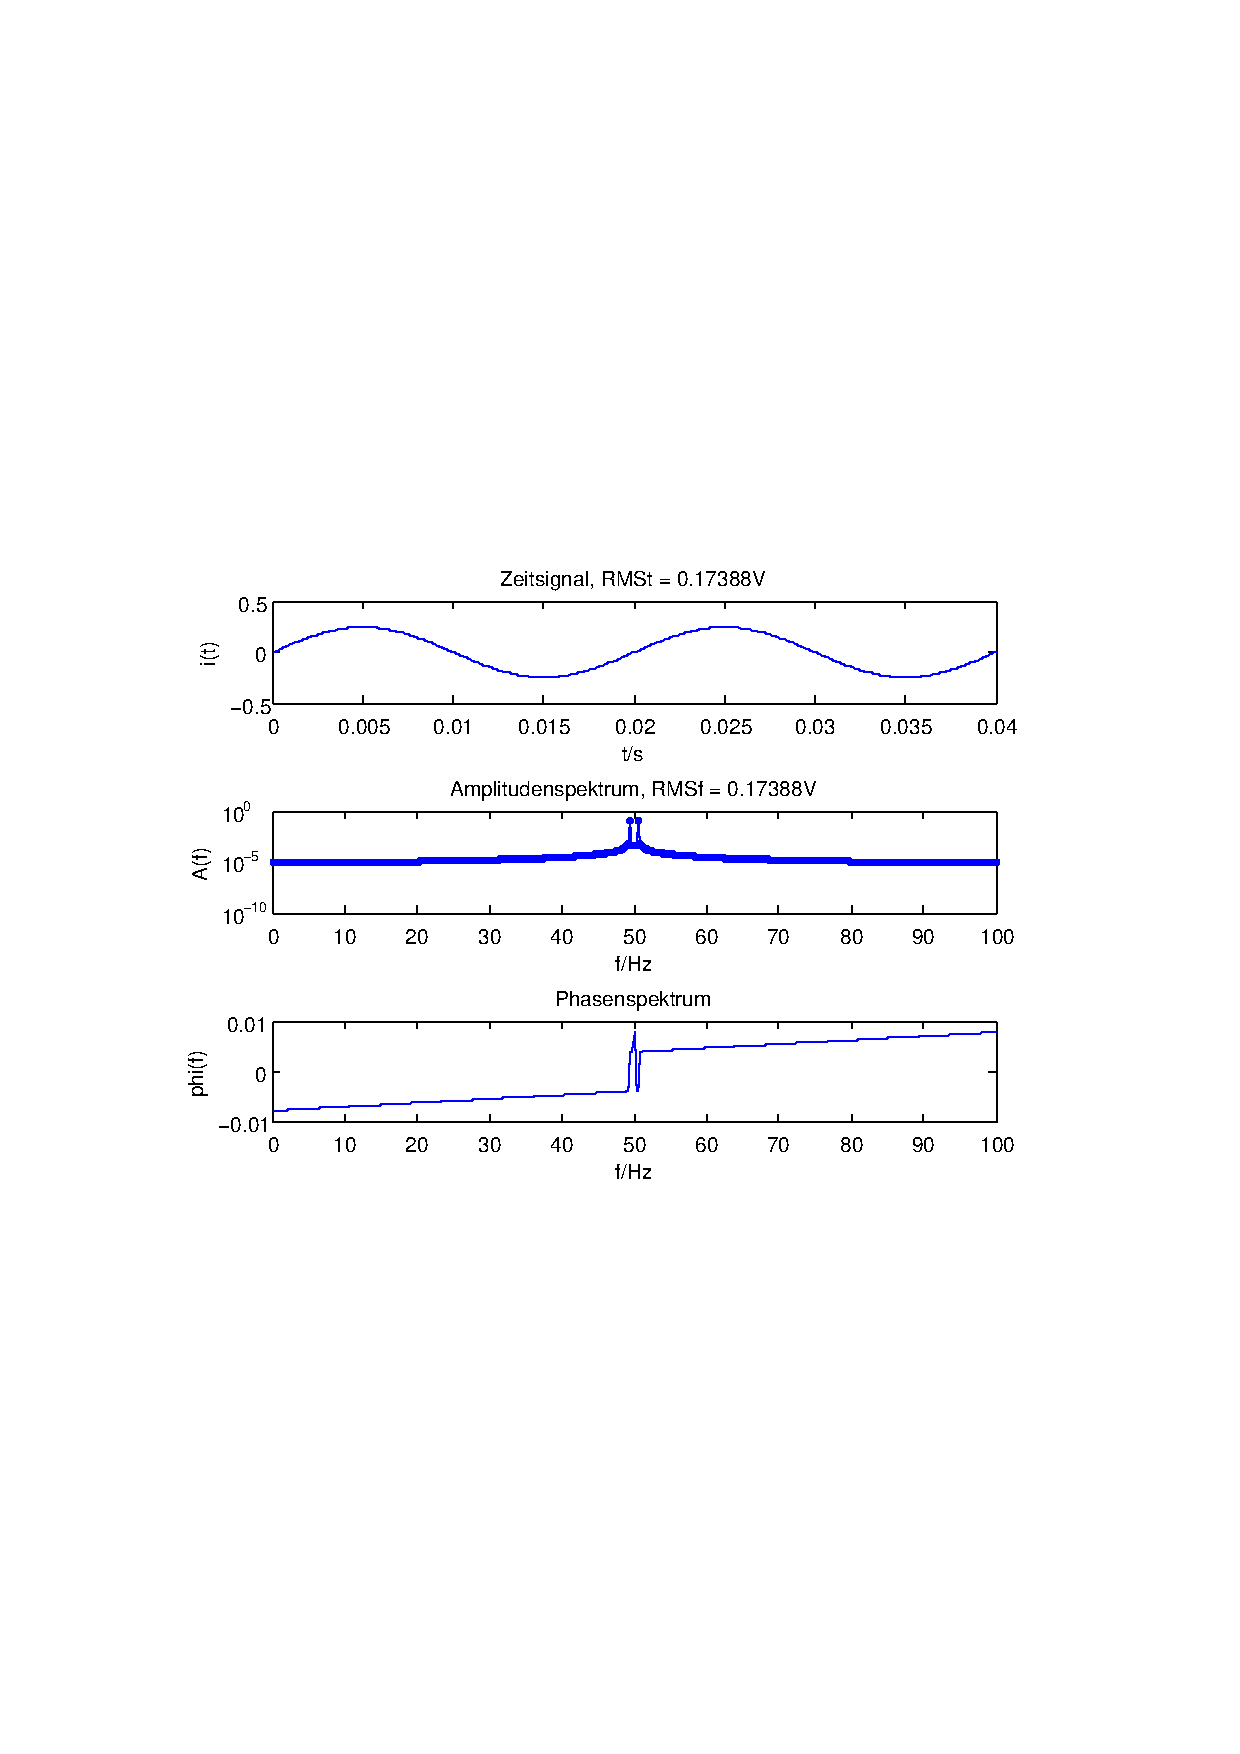
\includegraphics[scale=0.55, trim = 35mm 100mm 35mm 95mm, clip]{Bilder/sin_f-50_a-0}
                    \caption{Simulierte sinus-Funktion mit $\alpha = 0 \p 90^\circ$}
                \end{figure}
        
            \end{minipage}
        
            \begin{minipage}{0.6\textwidth}
                \begin{figure}[H]
                    \label{fig:pico_sin_f-50_a-00}
                    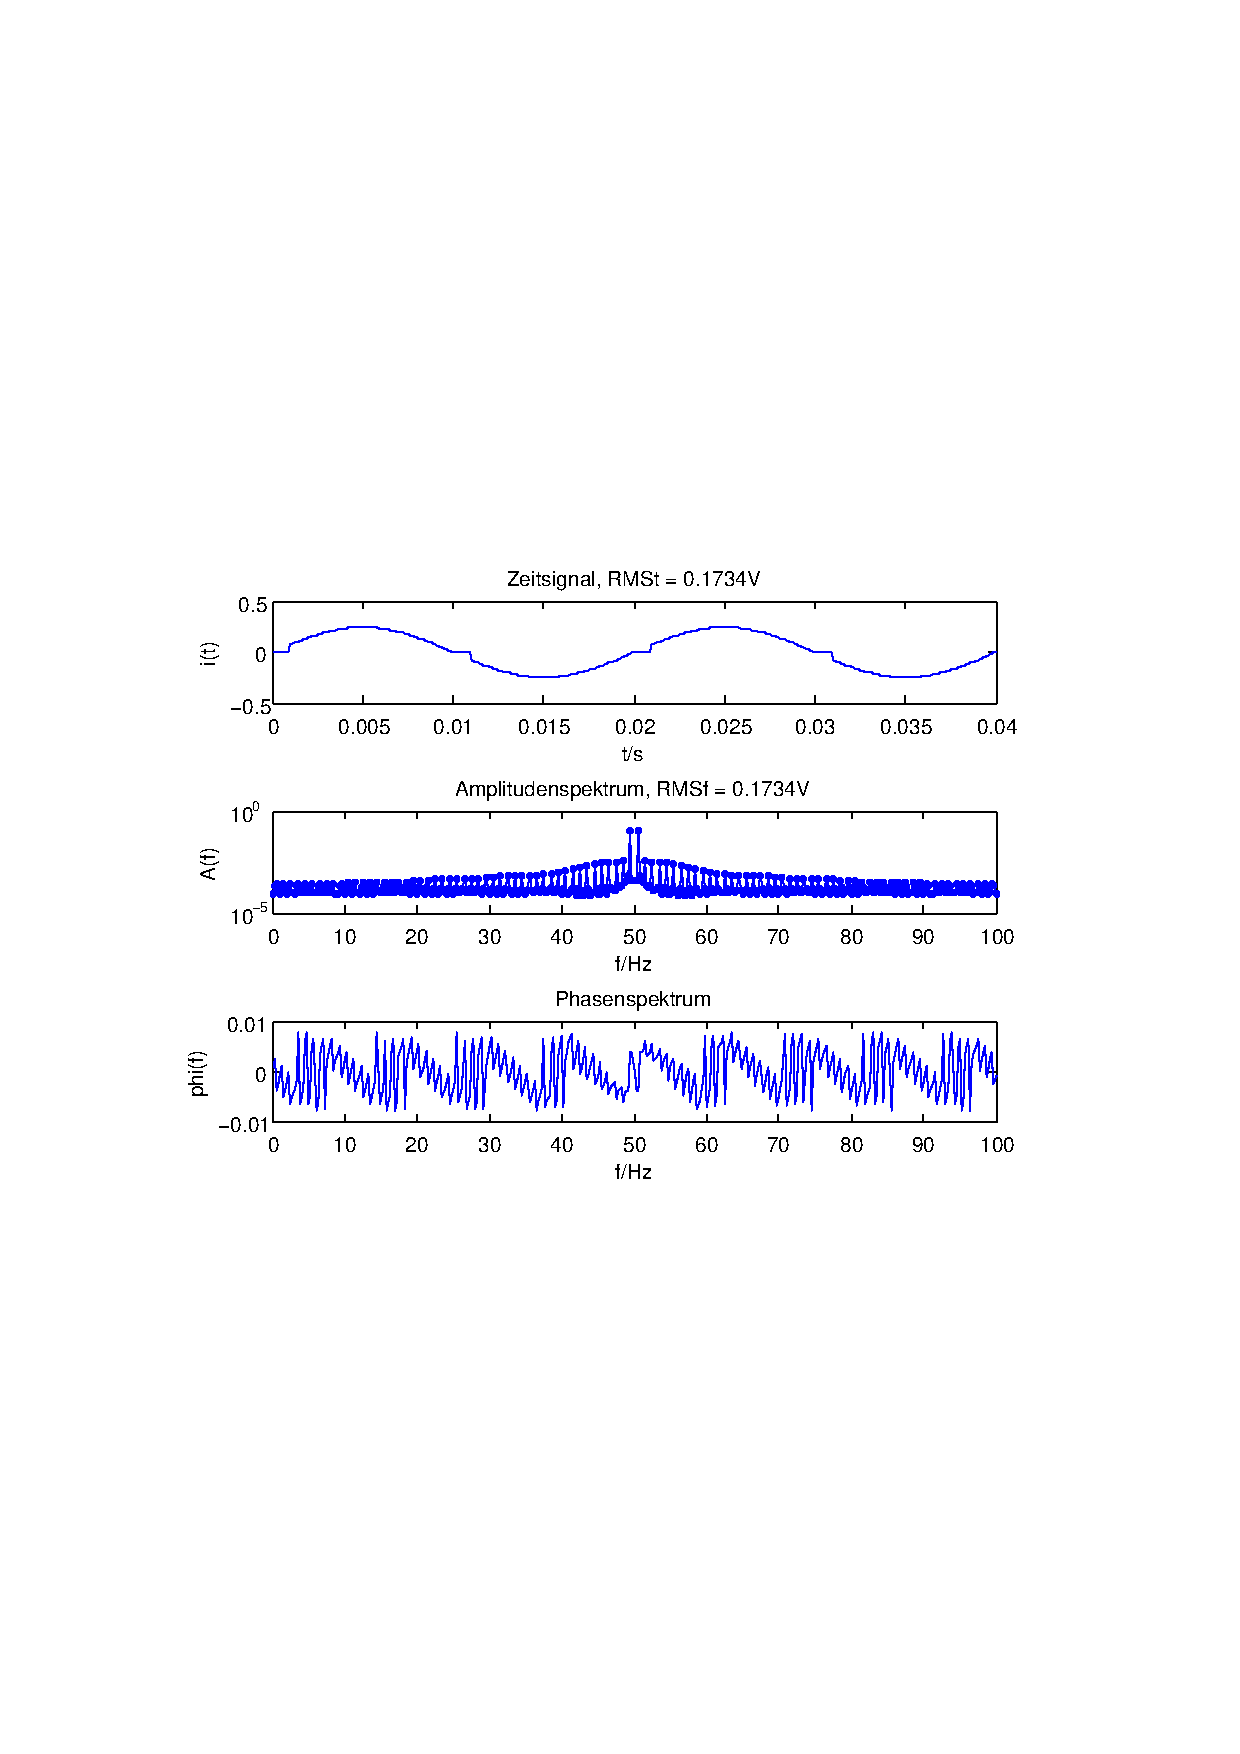
\includegraphics[scale=0.55, trim = 35mm 100mm 35mm 95mm, clip]{Bilder/sin_f-50_a-0,1}
                    \caption{Simuliert Sinus-Funktion mit $\alpha = 0,1 \p 90^\circ$}
                \end{figure}
        
            \end{minipage}
        
        \end{tabular}
        \end{center}




        \begin{center}
        \begin{tabular}{ll}
        
        \hspace{-2.5cm}
            \begin{minipage}{0.6\textwidth}
                
                \begin{figure}[H]
                    \label{fig:sin_f-50_a-0}
                    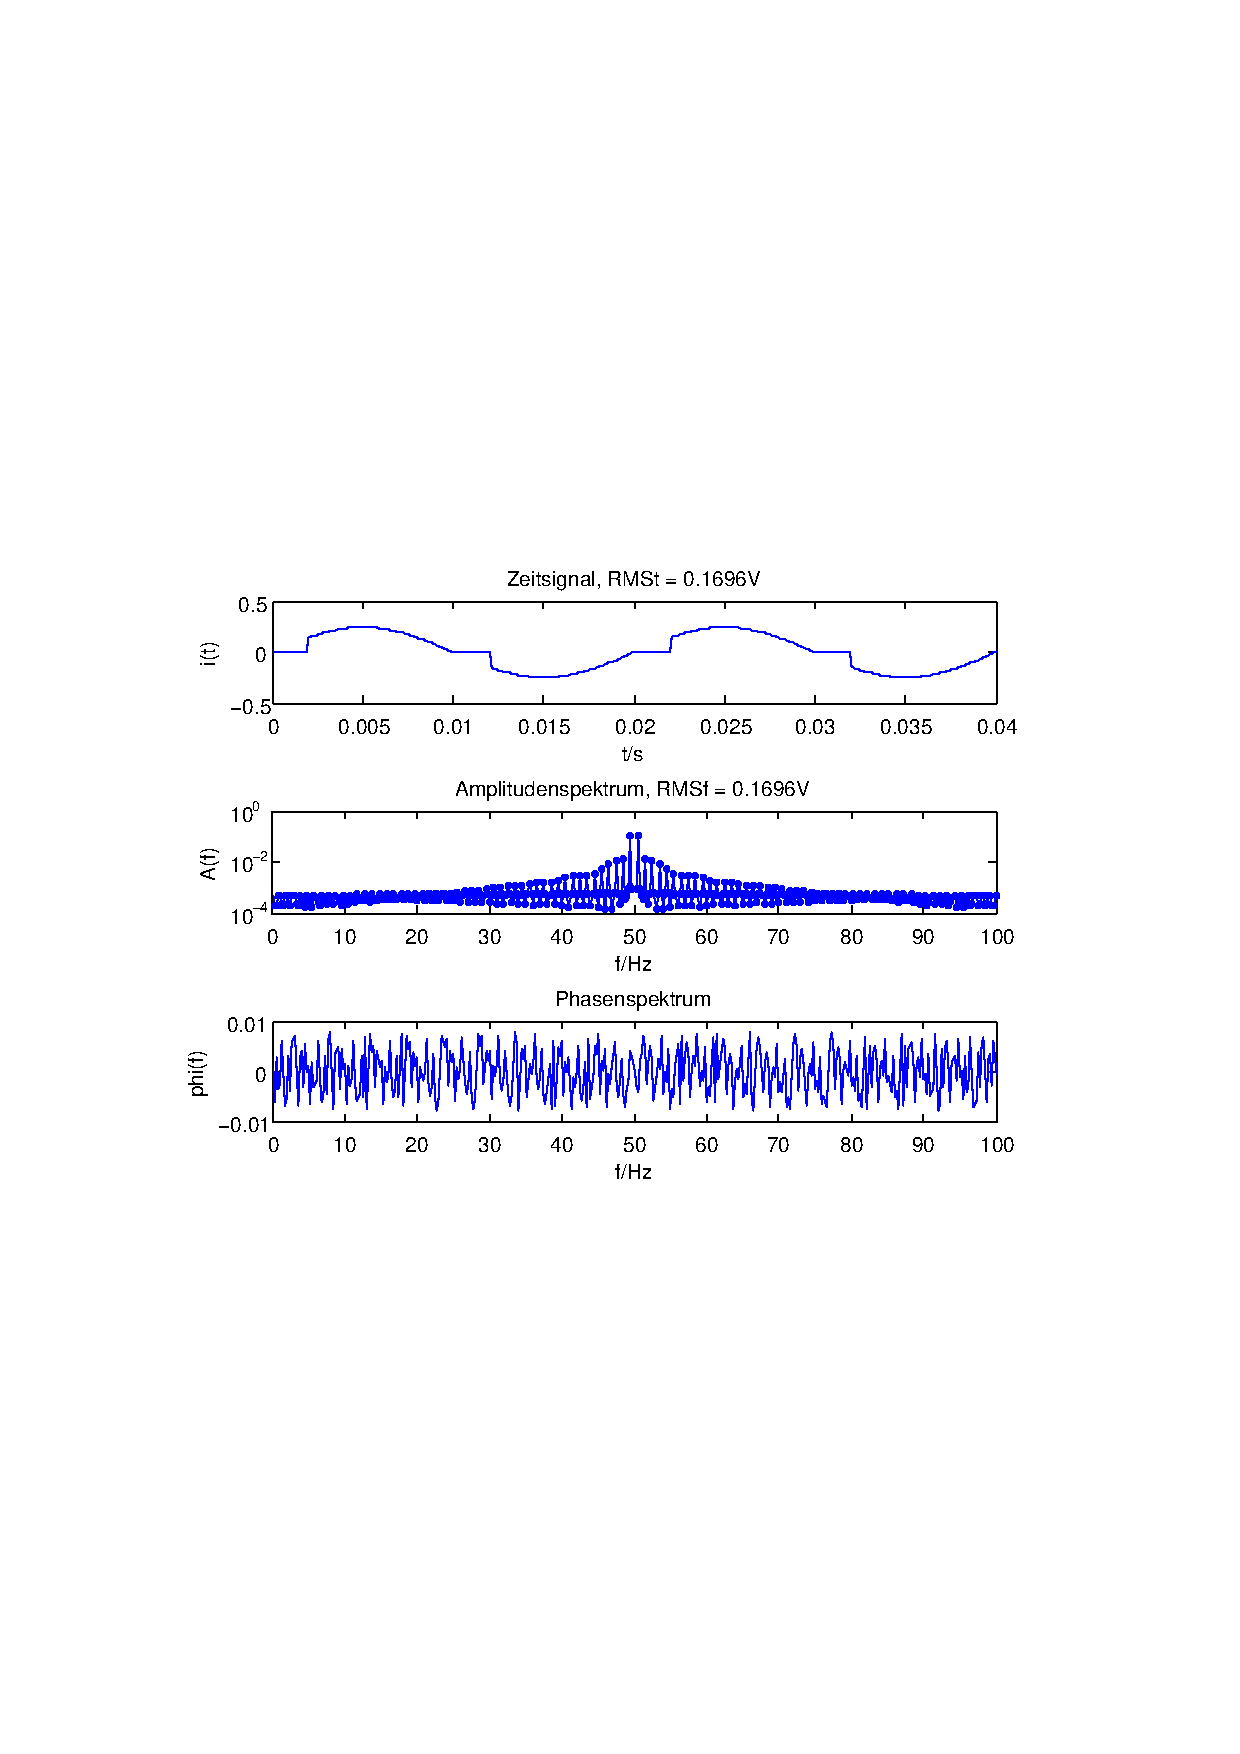
\includegraphics[scale=0.55, trim = 35mm 100mm 35mm 95mm, clip]{Bilder/sin_f-50_a-0,2}
                    \caption{Simulierte sinus-Funktion mit $\alpha = 0,2 \p 90^\circ$}
                \end{figure}
        
            \end{minipage}
        
            \begin{minipage}{0.6\textwidth}
                \begin{figure}[H]
                    \label{fig:pico_sin_f-50_a-00}
                    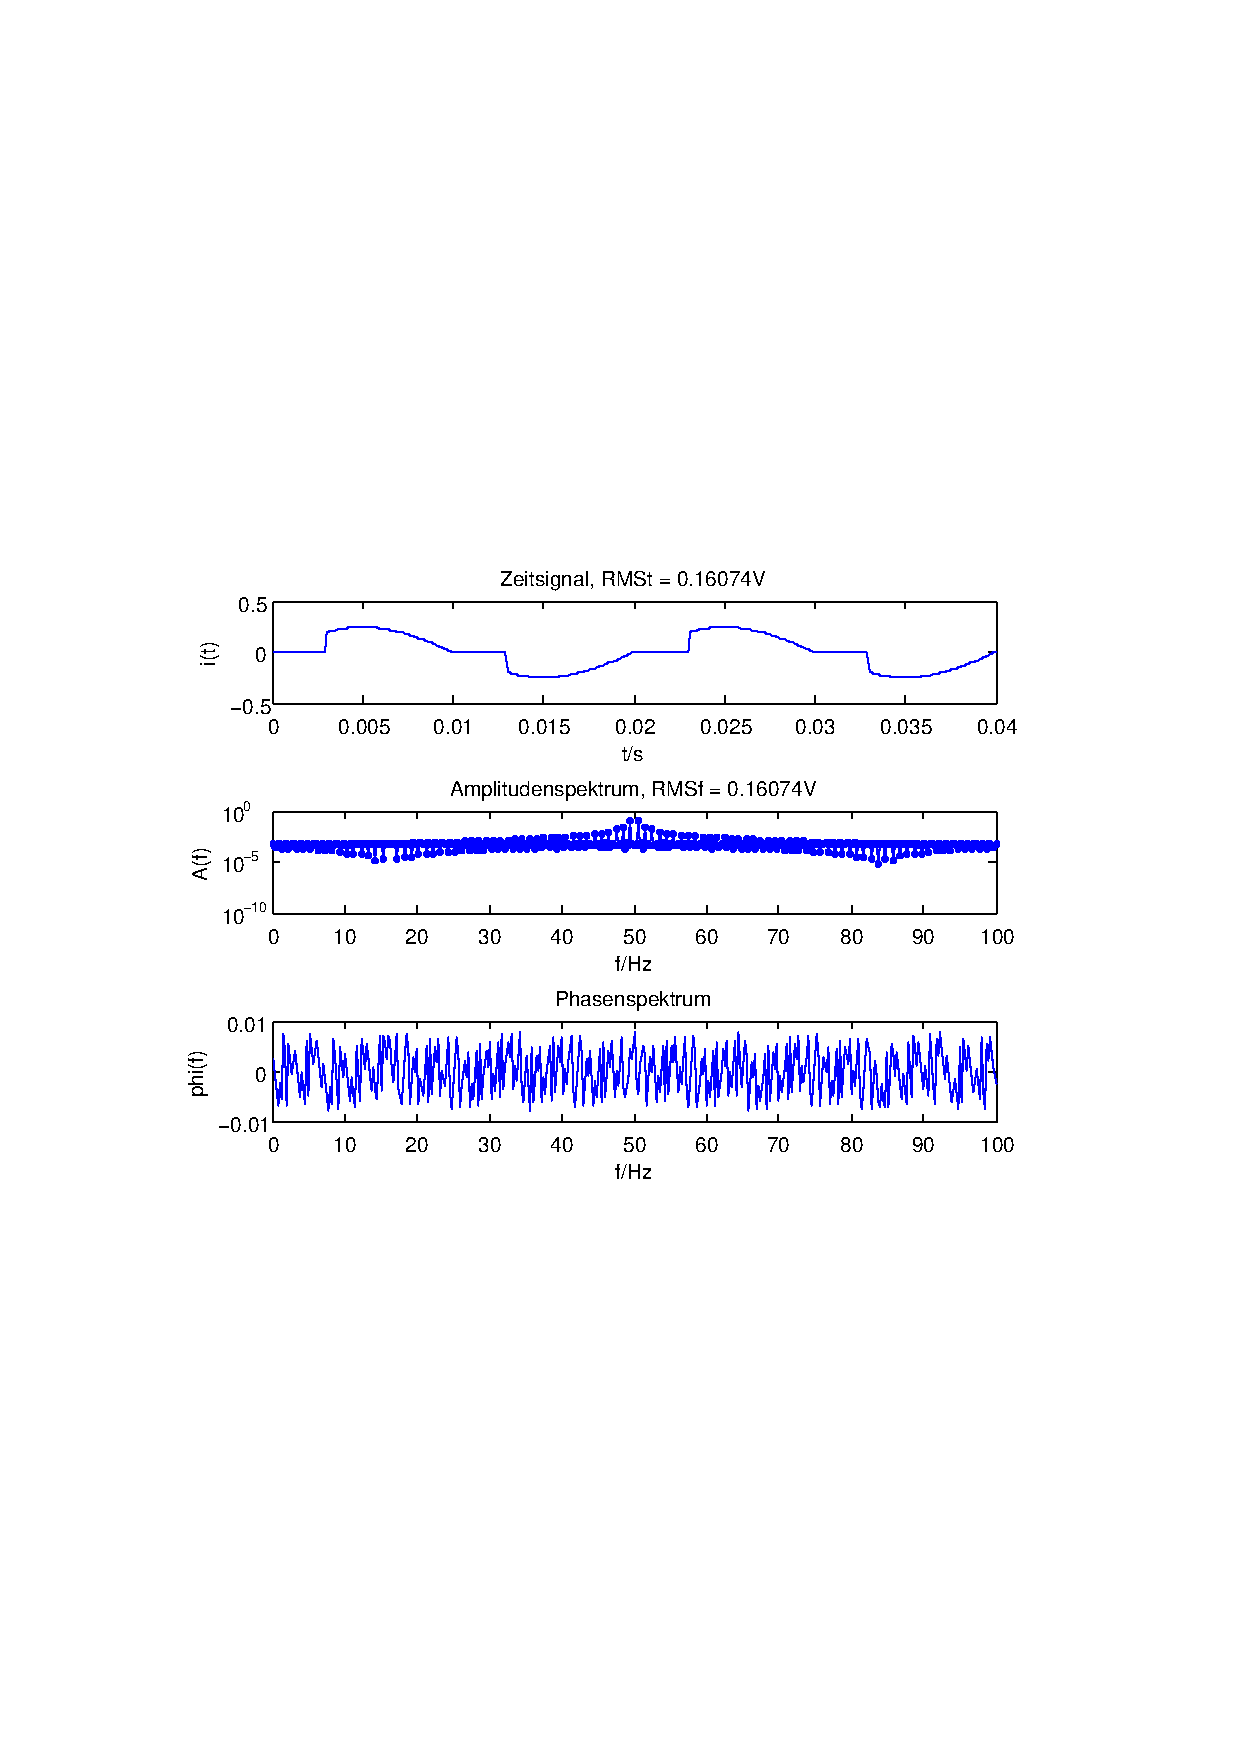
\includegraphics[scale=0.55, trim = 35mm 100mm 35mm 95mm, clip]{Bilder/sin_f-50_a-0,3}
                    \caption{Simuliert Sinus-Funktion mit $\alpha = 0,3 \p 90^\circ$}
                \end{figure}
        
            \end{minipage}
        
        \end{tabular}
        \end{center}





        \begin{center}
        \begin{tabular}{ll}
        
        \hspace{-2.5cm}
            \begin{minipage}{0.6\textwidth}
                
                \begin{figure}[H]
                    \label{fig:sin_f-50_a-0}
                    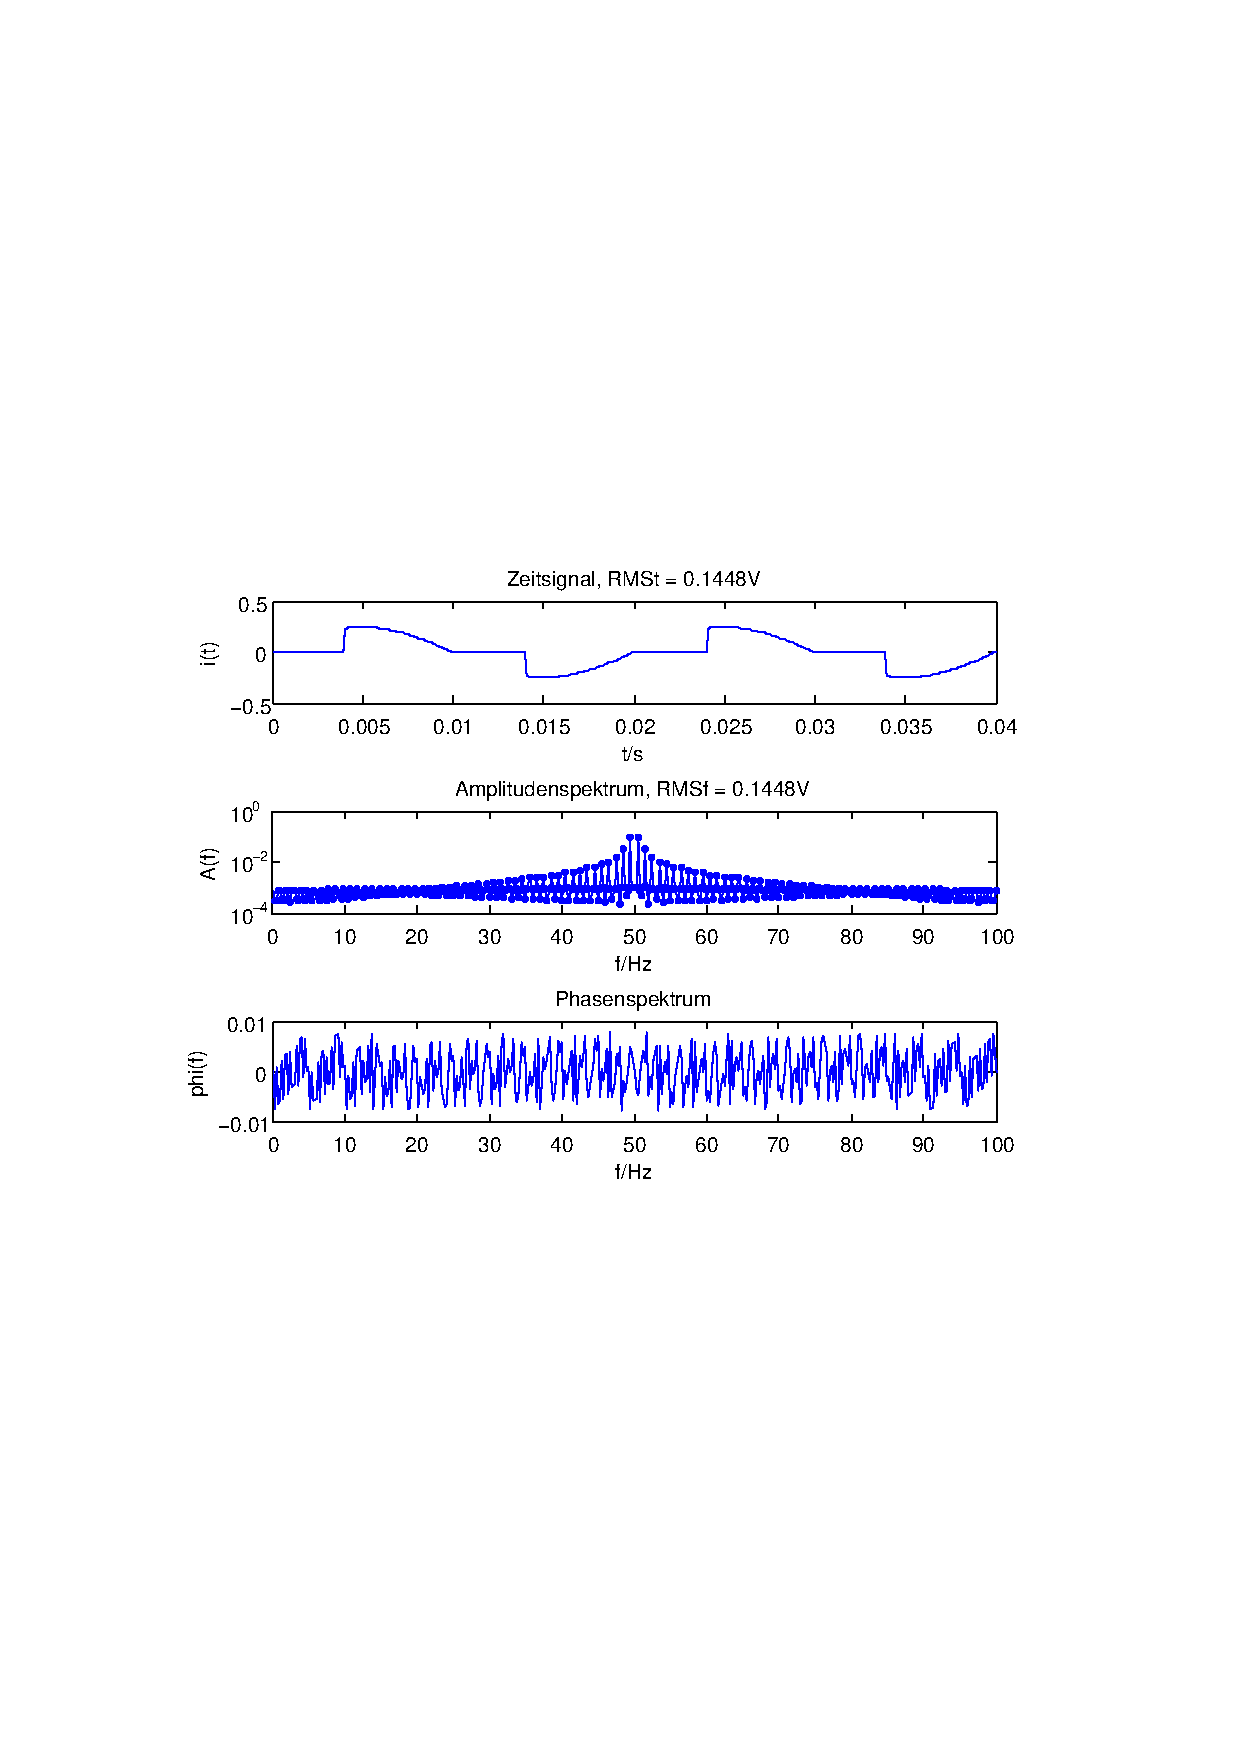
\includegraphics[scale=0.55, trim = 35mm 100mm 35mm 95mm, clip]{Bilder/sin_f-50_a-0,4}
                    \caption{Simulierte sinus-Funktion mit $\alpha = 0,4 \p 90^\circ$}
                \end{figure}
        
            \end{minipage}
        
            \begin{minipage}{0.6\textwidth}
                \begin{figure}[H]
                    \label{fig:pico_sin_f-50_a-00}
                    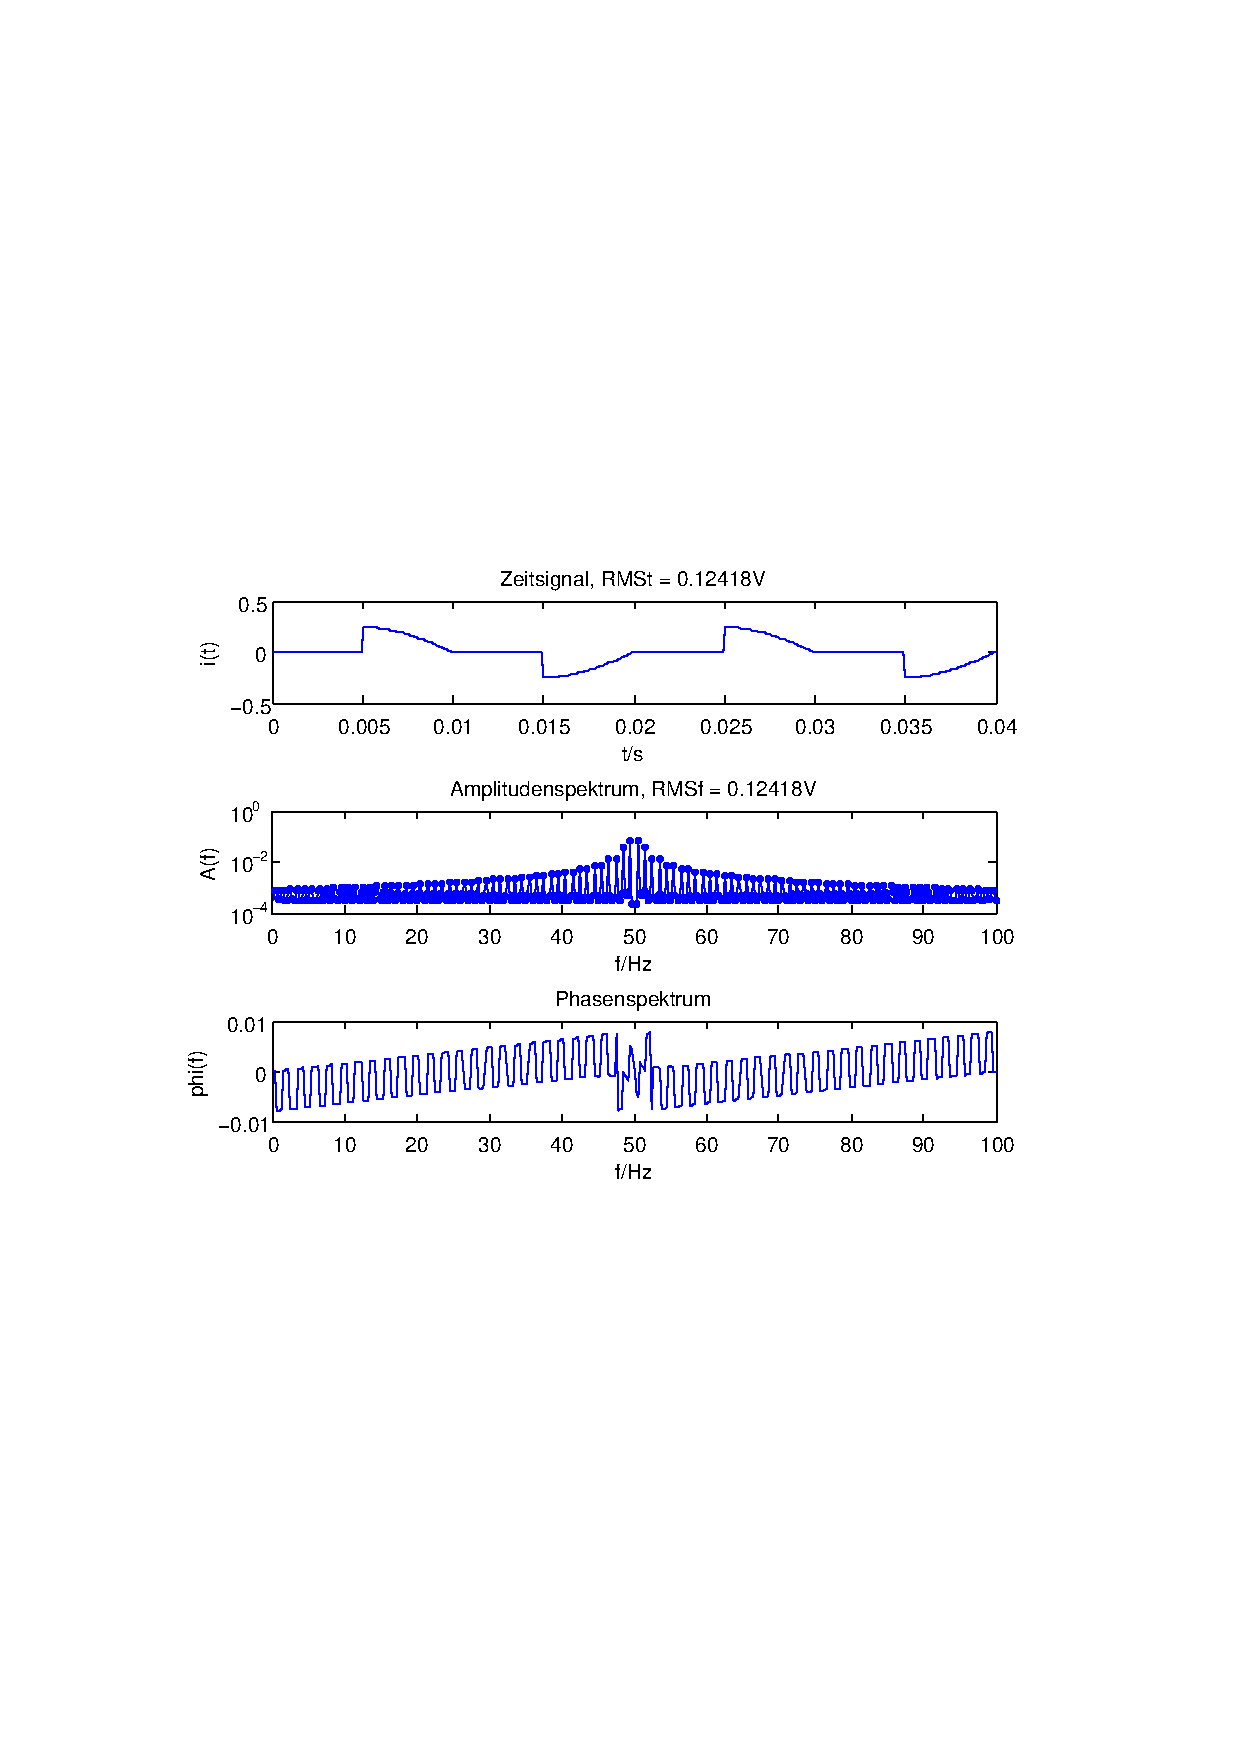
\includegraphics[scale=0.55, trim = 35mm 100mm 35mm 95mm, clip]{Bilder/sin_f-50_a-0,5}
                    \caption{Simuliert Sinus-Funktion mit $\alpha = 0,5 \p 90^\circ$}
                \end{figure}
        
            \end{minipage}
        
        \end{tabular}
        \end{center}


        Es ist zu beobachten, dass der Effektivwert mit zunehmendem Alpha sinkt und die Lampe somit gedimmt wird.\\
        Die RMS Werte im Zeit- und Frequenzbereich sind jeweils die selben.


\subsection{Matlab-Code}
    \begin{quote}
        
        \lstinputlisting[
            caption={Matlab-script},
            label=lst:Matlab]
            {./Matlab/vorbereitung.m}
            
            \lstinputlisting[
            caption={Matlab-script},
            label=lst:Matlab]
            {./Matlab/stromPhasSchnitt.m}
        
        \lstinputlisting[
            caption={Matlab-script},
            label=lst:Matlab]
            {./Matlab/EffektivwertZeitbereich.m}


        \lstinputlisting[
            caption={Matlab-script},
            label=lst:Matlab]
            {./Matlab/EffektivwertFourier.m}


    \end{quote}


    


\end{quote}

%--------------------------------------------------------------------
%--------------------------------------------------------------------





%--------------------------------------------------------------------
%--------------------------------------------------------------------
% \begin{thebibliography}{999}
% 
% \bibitem{krachler}Christian Krachler:
% \href{http://www.krachler.com/fileadmin/user_upload/arbeiten/Reglersynthese_Christian_Krachler.pdf}{Reglersynthese nach dem Frequenzkennlinienverfahren}, S16, S22, 08.05.2012
% 
% 
% %Name, Vorname.; evtl. Name2, Vorname2.: Titel des Dokumentes
% %oder Buches, Zeitschrift/Verlag/URL (Auflage, Erscheinungsort, -jahr), ggf. Seitenzahlen
% %\bibitem [Wiki10] {DigitaleMesskette2} \url{www.wikipedia.org}, Zugriff 22.03.2010
% \end{thebibliography}


\end{document}
